\documentclass[12pt, openright, oneside, a4paper, brazil]{abntex2}
\usepackage{lmodern}
\usepackage[T1]{fontenc}		% Selecao de codigos de fonte.
\usepackage[utf8]{inputenc}
\usepackage{nameref}
\usepackage[justification=justified,singlelinecheck=false]{caption}
\usepackage{lastpage}
\usepackage{amsmath}
\usepackage{indentfirst}
\usepackage{color}				% Controle das c ores
\usepackage{graphicx}			% Inclusão de gráficos
\usepackage{microtype} 			% para melhorias de justificação
\usepackage[brazilian,hyperpageref]{backref}	 % Paginas com as citações na bibl
\usepackage[alf, abnt-emphasize=bf, abnt-url-package=none, abnt-repeated-title-omit=yes, abnt-full-initials=yes, abnt-etal-list=3, abnt-etal-text=emph]{abntex2cite} % Citações padrão ABNT
\usepackage{trabalho}	% Citações padrão ABNT
\usepackage{lipsum}				% para geração de dummy text
\usepackage{trivfloat} 	%Quadros
% ---

% ---
% Pacotes de citações
% ---

% ---
% CONFIGURAÇÕES DE PACOTES

% Quadro
\trivfloat{quadro}
\renewcommand{\listquadroname}{Lista de Quadros}
\renewcommand{\backrefpagesname}{Citado na(s) página(s):~}
\renewcommand{\backref}{}
\renewcommand*{\backrefalt}[4]{
	\ifcase #1 %
		Nenhuma citação no texto.%
	\or
		Citado na página #2.%
	\else
		Citado #1 vezes nas páginas #2.%
	\fi}%

\titulo{UMA API WEB ORIENTADA A METADADOS COMO SERVIÇO DE RECOMENDAÇÃO HÍBRIDA}
\autor{Iury Krieger}
\local{\vfill Videira - Santa Catarina}
\data{2017}
\orientador{Msc. Tiago Heineck}
\coorientador{Msc. Wanderson Rigo}
\instituicao{
  Instituto Federal Catarinense - Câmpus Videira
  \par
  Bacharelado em Ciência da Computação
  }
\tipotrabalho{Trabalho de conclusão de curso}
\preambulo{Trabalho de conclusão de curso submetido ao Instituto Federal Catarinense - Câmpus Videira como parte dos requisitos para a obtenção do grau de Bacharel em Ciência da Computação}

\makeatletter
\hypersetup{
		pdftitle={\@title},
		pdfauthor={\@author},
    	pdfsubject={\imprimirpreambulo},
	    pdfcreator={LaTeX with abnTeX2},
		pdfkeywords={abnt}{latex}{abntex}{abntex2}{trabalho acadêmico},
		colorlinks=true,       		% false: boxed links; true: colored links
    	linkcolor=blue,          	% color of internal links
    	citecolor=blue,        		% color of links to bibliography
    	filecolor=magenta,      		% color of file links
		urlcolor=blue,
		bookmarksdepth=4
}
\makeatother
\setlength{\parindent}{1.3cm}
\setlength{\parskip}{0.2cm}
\makeindex

\begin{document}
\frenchspacing
\imprimircapa
\imprimirfolhaderosto

\begin{comment}
\begin{folhadeaprovacao}
	\begin{figure}[htb]
		\begin{center}
			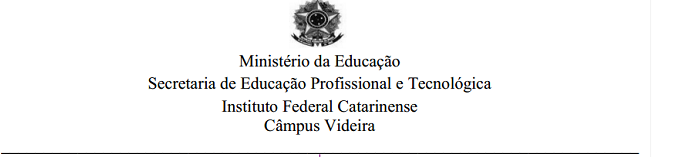
\includegraphics{images/logo.png}
		\end{center}
	\end{figure}
	{\ABNTEXchapterfont\large{\textbf{BACHARELADO EM CIÊNCIA DA COMPUTAÇÃO}}}
	\begin{center}
		{\ABNTEXchapterfont\large\imprimirautor}

		\vspace*{\fill}\vspace*{\fill}
		\begin{center}
			\ABNTEXchapterfont\bfseries\Large\imprimirtitulo
		\end{center}
		\vspace*{\fill}
	\end{center}

	Este Trabalho de Conclusão de Curso foi julgado adequado para a obtenção do título de Nome do Título em Nome do Curso, Área de Concentração e aprovada em sua forma final pelo Curso de Nome do Curso

	\assinatura{\textbf{\imprimirorientador} \\ Orientador}
	\assinatura{\textbf{Msc. Marcelo Cendron} \\ Professor Convidado I}
	\assinatura{\textbf{Maurício Ferreira} \\ Professor Convidado II}

	\begin{center}
		\vspace*{0.5cm}
		{\large\imprimirlocal}
		\par
		{\large\imprimirdata}
		\vspace*{1cm}
	\end{center}
\end{folhadeaprovacao}
\end{comment}

\begin{folhadeaprovacao}

  \begin{center}
  \vspace*{-1.2cm}
    {\large\imprimirautor}

    \vspace*{\fill}\vspace*{\fill}\vspace*{\fill}
    {\large\imprimirtitulo}
    \vspace*{\fill}\vspace*{\fill}

    \hspace{.45\textwidth}
    \begin{minipage}{.5\textwidth}
        \imprimirpreambulo
    \end{minipage}%
    \vspace*{\fill}
   \end{center}

  \begin{center}
  	 Videira (SC), 16 de Maio de 2017
  \end{center}

    \vspace{-1cm}

   \assinatura{\begin{center}\vspace{-0.6cm}\imprimirorientador \\
   					   Instituto Federal Catarinense
   					   \end{center}
   	}
   	\assinatura{\begin{center}\vspace{-0.6cm} Msc. Wanderson Rigo \\
   					   Instituto Federal Catarinense
   					   \end{center}
   	}
    \begin{center}
  	\textbf{BANCA EXAMINADORA}
   \end{center}
   \vspace{-1cm}
   \assinatura{\begin{center}\vspace{-0.6cm} Msc. Marcelo Cendron \\
      					   Instituto Federal Catarinense
   					     \end{center}
   }
   \assinatura{\begin{center}\vspace{-0.6cm}Maurício Ferreira \\
       					   Instituto Federal Catarinense
   					    \end{center}
    }

    \vspace*{1cm}

\end{folhadeaprovacao}

\setlength{\absparsep}{18pt} % ajusta o espaçamento dos parágrafos do resumo
\begin{resumo} 

Devido a expansão massiva de dados produzidos e disponíveis na Internet, os usuários estão cada vez mais sobrecarregados de informação, não sabendo distinguir informações realmente úteis. Para sanar este problema, os sistemas de recomendação visam recomendar os itens mais úteis a cada usuário, através de técnicas de machine learning. Tais técnicas visam prever a avaliação de um usuário a um item, baseando-se nas avaliações já conhecidas. Este trabalho propõe o desenvolvimento de uma API Web de código aberto que recomenda itens a usuários, fazendo uso de um sistema de recomendação híbrido que analisa as estruturas pré definidas e proporciona recomendações, baseando-se nos metadados fornecidos, através do conteúdo do item e da filtragem colaborativa de usuários. Tal sistema poderá processar suas recomendações utilizando a GPU, minimizando o tempo da requisição de recomendação e consequentemente aumentando a eficiência da aplicação. Dessa forma é possível fornecer um serviço multi-propósito desprendido de qualquer ambiente e linguagem de programação, trazendo uma visão mais transparente dos sistemas de recomendação aos desenvolvedores.

\textbf{Palavras-chaves}: Sistemas de Recomendação. Aprendizado de Máquina. Metadados. Computação em GPU.
\end{resumo}

\begin{resumo}[Abstract]
 \begin{otherlanguage*}{english}

Due to the massive expansion of data produced and available on the Internet, users are increasingly overloaded with information, not knowing how to distinguish which is really useful. To remedy this problem, recommendation systems aim to recommend the most useful items to each user through machine learning techniques. These techniques are intended to predict a user's rating of an item, based on previously known rating. This work proposes the development of an open-source Web API that recommends items to users, making use of a hybrid recommendation system that analyzes the pre-defined structures and provides recommendations, based on the metadata provided, through item content and collaborative filtering. Such a system can process its recommendations using the GPU, minimizing the time of the recommendation request and consequently increasing the application efficiency. Therefore is possible to provide a multi-purpose service detached from any environment and programming language, bringing a more transparent view of recommendation systems to developers.

  \textbf{key-words}: Recommender Systems. Machine Learning. Metadata. GPU Computing.
 \end{otherlanguage*}
\end{resumo}

% ---
% Lista de quadros
% ---
\counterwithout{quadro}{chapter}
\newpage % Forçar a lista de quadros em uma nova página
\phantomsection % Comando necessário caso o pacote hyperref seja utilizado, visando a corrigir o link
\pdfbookmark[0]{\listofquadros}{lof}
\listofquadros* % Adiciona lista de quadros
\cleardoublepage

% ---
% Lista de figuras
% ---
\pdfbookmark[0]{\listfigurename}{lof}
\listoffigures*
\cleardoublepage

% ---
% Siglas
% ---
\begin{siglas}

	\item[IA]{\textit{Inteligência Artificial}}
	\item[HTTP]{\textit{Hypertext Transfer Protocol}}
	\item[API]{\textit{Application Program Interface}}
	\item[REST]{\textit{Representational State Transfer}}
	\item[JSON]{\textit{Javasript Object Notation}}

\end{siglas}

% ---
% Sumário
% ---
\pdfbookmark[0]{\contentsname}{toc}
\tableofcontents*
\textual

\chapter{INTRODUÇÃO}

Com o avanço crescente do campo tecnológico, os computadores vêm desempenhando tarefas antes incumbidas à seres humanos. O poder de computação provou-se muito eficaz ao desempenhar tarefas que possuíssem um padrão possível de se expressar através de um algoritmo, mais ainda, se este padrão fosse repetitivo.

Logo os computadores começaram a desempenhar funções nas mais diversas áreas, desde cálculos matemáticos à manipulação de imagens. Atualmente, das funções desempenhadas pelos computadores, a mais difícil de se reproduzir com precisão é o padrão de raciocínio humano.

Alguns autores defendem que para que um computador atinja tal nível, seria necessário que o mesmo possuísse consciência, assim como os seres humanos. Outros defendem que o raciocínio humano não consegue ser reproduzido, apenas emulado, devido à impossibilidade de se programar uma consciência computacional. Tal área de estudo, que tem como o foco o desenvolvimento de sistemas computacionais rumo a proximidade do método humano, chama-se inteligência artificial \cite{russell2004inteligencia, coppin2015inteligencia}.

Possível ou não, é inegável o avanço da inteligência artificial desde seu início nos primórdios da computação. Algumas tarefas, tais como a atribuição de uma consciência a um sistema computacional, deixaram de ser o foco da área, uma vez que não possuímos a tecnologia para construir sistemas muito mais complexos que os atuais  \cite{russell2004inteligencia}.

Entretanto, a inteligência artificial encontrou-se muito eficaz em outras áreas do método humano, tais como o aprendizado, um dos segmentos mais importantes da área, dentro da inteligência artificial chamado de aprendizado de máquina (\textit{machine learning}) \cite{coppin2015inteligencia}.

Desde os anos 90 a preocupação com o armazenamento e a expansão massiva de dados produzidos já existia, prevendo que usuários ficariam sobrecarregados de informação, não sabendo distinguir o que seria realmente útil \cite{hill1995recommending, adomavicius2005toward}. Na época, uma comunidade virtual de avaliação foi proposta para proporcionar aos usuários o mínimo de esforço ao encontrar informações úteis. Com a evolução da inteligência artificial e das técnicas de machine learning, este trabalho de avaliação e recomendação, antes feito por uma comunidade, hoje é atribuído aos sistemas de recomendação \cite{hill1995recommending}.

Sistemas de recomendação (RSs) são ferramentas de  software e técnicas que provém sugestões de artefatos à usuários. Estes artefatos são definidos como os objetos de valor à serem recomendados \cite{ricci2011introduction}. Atualmente, o interesse em tais sistemas se mantém alto, devido a abundância de aplicações práticas \cite{adomavicius2005toward}, exemplificadas nos casos de \textit{E-commerce} por \citeonline{schafer2001commerce}, além de \citeonline{linden2003amazon}, onde são amplamente utilizados.

Desta forma, sistemas de recomendação vem sendo desenvolvidos para a resolução do problema descrito nas mais diversas áreas \cite{bennett2007netflix, gavalas2014mobile}, desde aplicações hoteleiras como o TripAdvisor até aplicações de entretenimento como a Netflix, além da sua origem nos \textit{E-commerces} citados anteriormente. Muitos destes sistemas são casos de RSs aplicados a itens e finalidades específicas \cite{huang2002graph, brozovsky2007recommender}, onde todo o motor de recomendação segue uma abordagem baseada no padrão que lhe foi dado.

Por outro lado, ao observar aplicações web de sistemas de recomendação, verifica-se a existência de soluções em forma de APIs, tais como o Google Cloud Platform e o Microsoft Cognitive Services, fornecidas como serviços transparentes. Entretanto, estas soluções proprietárias não são incorporadas a aplicação, mas sim utilizadas como serviços externos, dificultando a personalização.

Para sanar estes problemas, este trabalho propõe o desenvolvimento de uma API que proporcione uma visão mais transparente dos sistemas de recomendação, permitindo ao usuário desfrutar das funcionalidades, sem a necessidade de um profundo conhecimento dos detalhes que compõem as diferentes técnicas de recomendação, além dos problemas decorrentes do uso de cada uma das técnicas. Além disso, tal tecnologia será fornecida como um serviço de código aberto, podendo ser utilizada em qualquer ambiente.

Este trabalho está dividido em seis seções. A segunda seção apresenta o referencial teórico necessário para o entendimento total do escopo do trabalho. Na terceira seção são apresentadas as principais características do trabalho proposto, além de compará-lo com outros trabalhos relacionados. Em seguida, a quarta seção apresenta a metodologia a ser utilizada para realização do trabalho proposto na seção anterior. Mais à frente, na seção cinco, será abordado o cronograma a ser empregado para a realização do trabalho e, por fim, na sexta seção são apresentadas as considerações finais.

\section{Objetivos}

\subsection{Objetivo Geral}

Desenvolver uma API web de código aberto para recomendação híbrida de itens a usuários.

\subsection{Objetivos Específicos}

\begin{itemize}

	\item Fornecer uma documentação das funcionalidades visando futura colaboração da comunidade e utilização por outros desenvolvedores.
	\item Proporcionar a recomendação das propriedades relevantes através das estruturas de metadados fornecidas.
	\item Possibilitar o processamento paralelo das recomendações em GPU.

\end{itemize}

\section{Metodologia}

A metodologia deste trabalho está dividida em três seções. Primeiramente serão implementadas todas as funcionalidades descritas anteriormente. Mais à frente, será feita a validação das funcionalidades implementadas e da eficácia das recomendações. Por fim, serão feitos os ajustes e correções necessárias de acordo com o resultado da validação das funcionalidades implementadas.

\subsection{Implementação}

Inicialmente serão implementados os algoritmos de recomendação híbrida, incluindo o processamento dos metadados fornecidos. Os algoritmos de recomendação resumem a eficácia da API e devem consumir a maior parte do tempo de desenvolvimento.

Ao completar a implementação das técnicas híbridas de sistemas de recomendação, serão implementadas as demais funcionalidades da API. Serão consideradas a identificação e entrada dos metadados, além do formato dos dados de saída.

Ao fim do desenvolvimento, o código será adaptado para processamento na GPU através de diretivas de compilação e bibliotecas especializadas.

\subsection{Validação}

Assim que a API esteja em um grau considerado funcional, será feita a validação da eficácia ao recomendar as estruturas fornecidas através de grupos de testes definidos, uma técnica amplamente utilizada na validação de técnicas de machine learning.

A validação será feita utilizando um grupo separado dos  dados utilizados para testes, confrontando as recomendações feitas com o resultado esperado. Através desses resultados é medida a acurácia de um sistema de recomendação, métrica utilizada como medida de eficiência entre os diferentes métodos utilizados.

\subsection{Ajustes e Correções}

Por fim, serão feitos os ajustes e correções de erros recolhidos ao longo do processo, além de testar as funcionalidades e a utilização da API como um todo. A documentação será feita durante boa parte de todo o processo e, neste caso em específico, possui um foco especial, uma vez que o princípio da API é que a mesma seja utilizável por outros desenvolvedores, além de possibilitar a contribuição da comunidade.

\section{Trabalhos Relacionados}

Tendo como base as técnicas descritas acima, existem trabalhos como os apresentados por \citeonline{guo2015librec}, que abordam as técnicas em forma de biblioteca Java a ser incluída nos projetos. Esta abordagem torna a utilização mais simples devido ao fato do usuário poder utilizar apenas as funcionalidades da biblioteca, preocupando-se com o formato de entrada e saída dos dados, não com o processo de recomendação em si. Outra abordagem interessante é a proposta por \citeonline{brozovsky2007recommender} ao construir uma biblioteca C\# multi-propósito, focando na recomendação de itens com base na avaliação em um esquema de \textit{rating} (de uma a cinco estrelas), ou com base apenas em itens com avaliação positiva.

Do mesmo modo que a biblioteca desenvolvida por \citeonline{brozovsky2007recommender}, a API proposta neste trabalho também visa ser multi-propósito e distribuída como código aberto pela licença pública GNU (\textbf{GPL}), porém, fornecendo tais funcionalidades como um serviço web independente de linguagem de programação, o que não acontece nos exemplos apresentados.

Além dos trabalhos apresentados, \citeonline{do2013filtragem} aborda os sistemas de recomendação com uma perspectiva semelhante a este trabalho, focando mais no ganho de desempenho ao processar o método de filtragem colaborativa na GPU. Este trabalho não tem seu foco em desempenho, mas sim em uma proposta de \textbf{recomendação genérica}, que forneça recomendações a quaisquer modelos de usuários e itens através do método híbrido.

%
%--------- FIM INTRODUÇÃO------------
%

\cleardoublepage

\chapter{REFERENCIAL TEÓRICO}

\section{Aprendizado de Máquina}

Um dos segmentos da inteligência artificial com grande importância na atualidade é o aprendizado de máquina. Responsável pela construção de agentes capazes de, a partir de uma coleção de pares de entrada e saída, aprender uma função que prevê a saída para novas entradas. Tais agentes são definidos como tudo que pode perceber seu ambiente através de sensores, além de atuar sobre o mesmo através de atuadores. Em outras palavras, o aprendizado de máquina resume-se em técnicas que proporcionam a um algoritmo a capacidade de melhorar seu desempenho de forma automática, através do conhecimento obtido pelas entradas existentes \cite{coppin2015inteligencia}.

Dessa forma, considera-se que um agente está aprendendo se melhorar o seu desempenho nas tarefas para que foi designado, a partir de suas observações sobre o mundo. Este aprendizado proporciona às técnicas de \textit{machine learning} a capacidade evolutiva, uma vez que é possível não só responder as entradas do mundo exterior como também tirar conclusões sobre as mesmas, melhorando cada vez mais a natureza da solução \cite{russell2004inteligencia}.

Conforme apresentado por \citeonline{carbonell1983overview}, devido a capacidade de, além de solucionar problemas, melhorar automaticamente o desempenho da solução, os sistemas de aprendizagem tem suas aplicações nas mais diversas áreas, tais como agricultura, educação, sistemas especialistas de alta performance, reconhecimento de imagem, programação, etc. Através de um apanhado das aplicações nas áreas de utilização, \citeonline{carbonell1983overview} dividem o campo de aprendizado do \textit{machine learning} em três partes:

\begin{itemize}

	\item \textbf{Estudos orientados à tarefa (\textit{Task-oriented studies}):} composto pelo desenvolvimento e análise de sistemas de aprendizagem visando melhorar a performance na solução de determinadas tarefas.

	\item \textbf{Simulação cognitiva (\textit{Cognitive simulation}):} formado pela investigação e simulação do processo de aprendizagem humano.

	\item \textbf{Análise teórica (\textit{Theoretical analysis}):} exploração teórica do espaço de possíveis processos de aprendizado.

\end{itemize}

Analisando a taxonomia proposta por \citeonline{carbonell1983overview}, pode-se idenficar que o escopo deste trabalho encontra-se nos estudos orientados à tarefa, onde o propósito é a melhoria da performance, neste caso através de recomendações orientadas à metadados.

Como exemplo do uso das técnicas de \textit{machine learning}, \citeonline{sebastiani2002machine}  apresenta um algoritmo de categorização de texto que, a partir de um conjunto de documentos pré-classificados (entradas), constrói um classificador para novos documentos (novas entradas). Outro exemplo, apresentado por \citeonline{pang2002thumbs}, reforça a ideia de melhora de desempenho para novas entradas através de um padrão aprendido a partir de entradas já existentes. Através de dados sobre avaliações de filmes, pode-se perceber que, mesmo as técnicas padrão de \textit{machine learning}, acabam superando os patamares humanos na classificação de sentimentos.

\section{Sistemas de Recomendação}

Como ramificação do aprendizado de máquina, os sistemas de recomendação (RSs) são técnicas de software que provém sugestões a usuários de itens que os mesmos possam querer utilizar   \cite{resnick1997recommender, schafer1999recommender}. Desta forma, recomendações seriam, em sua forma mais simples, rankings de itens, tais como os utilizados na maioria das soluções de produtos (livros mais lidos, filmes mais assistidos, etc.) \cite{ricci2011introduction}. O que os RSs trazem de novo é a tentativa de predizer, através da filtragem colaborativa ou da similaridade de conteúdo, qual o ranking mais adequado de produtos ou serviços a um usuário. A filtragem colaborativa, termo cunhado por \citeonline{resnick1997recommender}, recomenda itens baseando-se nos relacionamentos do usuário. Por outro lado, a similaridade de conteúdo baseia-se no conteúdo de itens já avaliados pelo usuário. Tais dados podem ser coletadas de forma explícita, na forma de perguntas diretas e avaliações do usuário sobre os itens, ou de forma interpretativa, inferindo sobre ações tomadas pelo usuário e atribuindo peso a elas.

Mais formalmente, os sistemas de recomendação podem ser descritos matematicamente da seguinte forma: sendo \emph{C} o conjunto de todos os usuários e \emph{S} o conjunto de todos os itens que podem ser recomendados, tanto o espaço \emph{S} como o espaço \emph{C} podem ser extremamente grandes, batendo os milhões de usuários e itens \cite{adomavicius2005toward, gomez2016netflix}. Dessa forma, tem-se \textit{u} como a função de utilidade de um item \emph{s} para um usuário c. A função u utiliza-se do conjunto ordenado R, descrito como $C \times S \rightarrow R$, para encontrar o item $\emph{s} \in \emph{S}$ com a maior utilidade para o usuário \emph{c}. Um exemplo de como as preferências são armazenadas no espaço de avaliações C x S pode ser visto no quadro 1.

\begin{quadro}[h!tp]

	\caption{\label{movie_matrix}Exemplo de matriz de recomendações a filmes}

	\begin{center}
		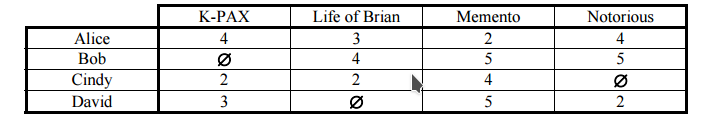
\includegraphics[scale=0.8]{images/movie_matrix.png}
	\end{center}

	\hspace{5.5cm}{Fonte: \citeonline{adomavicius2005toward}}

\end{quadro}

De acordo com o quadro 1, o símbolo "$\emptyset$" representa os filmes ainda não avaliados pelos usuários. Estes itens, por sua vez, são os alvos das técnicas de recomendação que tentam predizer a avaliação de um usuário. Uma vez que o motor de recomendação pode predizer as avaliações de um usuário, pode-se recomendar ao mesmo apenas os \emph{N} itens com a maior avaliação estimada \cite{adomavicius2005toward}.

Como consequência da importante participação dos sistemas de recomendação em sites com um grande número de público, tais como Netflix, eBay e Amazon.com, os mesmos tornaram-se ferramentas poderosas \cite{schafer1999recommender} e são considerados os propulsores de várias estatísticas, entre elas: o aumento da satisfação dos usuários, devido a precisão das recomendações; o aumento da fidelidade dos usuários, devido ao aumento de precisão quanto maior for a interação do usuário com o site; a aumento da capacidade do próprio serviço em entender melhor as intenções de seu público \cite{ricci2011introduction}. Tendo em vista o crescimento do número de aplicações que utilizam sistemas de recomendação e da variedade de soluções utilizadas em grandes sites, torna-se notável a importância dos mesmos.

Como próximo passo na evolução dos sistemas de recomendação, \citeonline{adomavicius2015context} propõem que os RSs, além de considerarem a similaridade entre perfis, devem estar cientes do contexto da avaliação do usuário ao construírem o modelo de perfil. Chamados de sistemas cientes de contexto, estes sistemas de recomendação devem diferenciar a ação que o usuário toma ao apenas analisar um item (filme, produto, etc.), não necessariamente indicando que itens parecidos devem ser recomendados no futuro, da ação tomada ao consumir um item (comprar, assistir, etc.). A partir dessa distinção de contexto, os RSs poderiam atribuir pesos diferentes para cada ação, podendo assim fazer recomendações mais precisas.

A seguir serão apresentados as diferentes técnicas dos sistemas de recomendação, além de qual técnica será utilizada por este trabalho e seus diferentes métodos através de algoritmos. Devido a existência de inúmeras técnicas e métodos de recomendação, este trabalho abordará apenas as técnicas necessárias para entendimento do mesmo, aprofundando-se apenas nos métodos que compõem a técnica utilizada.

\subsection{Método Baseado em Conteúdo}

Sistemas de recomendação que implementam o método baseado em conteúdo (\textit{content-based}) analisam um conjunto de documentos/descrições de itens previamente avaliados pelo usuário, construindo um modelo dos interesses baseando-se nas características dos itens avaliados \cite{mladenic1999text, adomavicius2005toward, lops2011content}. Este modelo serve para ser cruzado com o conteúdo de outros itens ainda não avaliados pelo usuário. Quanto maior o grau de semelhança entre o modelo do usuário e as características do item, maior a probabilidade do mesmo ter interesse.

Para que o modelo de interesses do usuário seja criado e confrontado com outros conteúdos ainda não avaliados, são necessários três atores principais que dividem a recomendação baseada em conteúdo: \textbf{analisador de conteúdo}, \textbf{aprendiz de perfis} e \textbf{componente de filtragem} \cite{lops2011content}. A estrutura completa destes agentes pode ser vista na figura 1.

\begin{figure}[h!tp]
	\caption{\label{content_based}Arquitetura de um sistema baseado em conteúdo}

	\begin{center}
		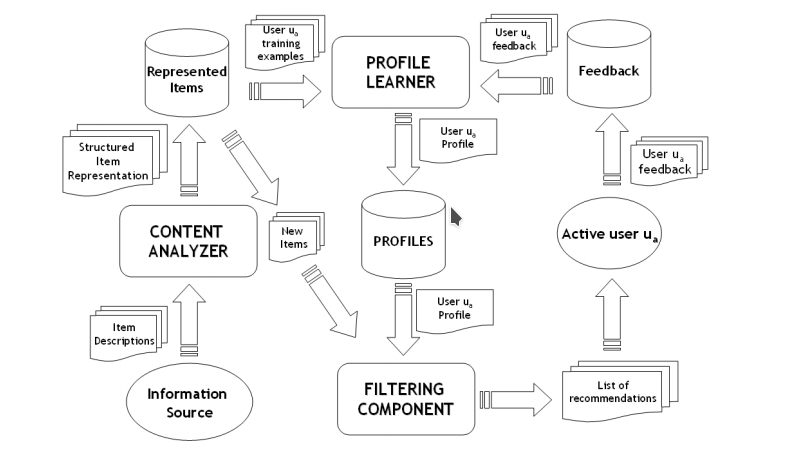
\includegraphics[scale=0.8]{images/content_based.png}
	\end{center}
	\hspace{5.5cm}{Fonte: \citeonline{lops2011content}}
\end{figure}

Note que na figura 1, a primeira parte do processo começa com o \textbf{analisador de conteúdo} (\textit{content analyzer}), transformando dados não estruturados em estruturas de atributos e características \cite{lops2011content, mladenic1999text}, armazenando-as no repositório de itens representados (\textit{represented items}). Para a construção e atualização do perfil de interesses do usuário ativo (representado na figura 1 por $u_{a}$), as avaliações do usuário para novos itens são armazenadas no repositório de feedback. O tipo de avaliação depende de cada aplicação, podendo ser expressado de forma \textbf{explícita}, como as avaliações binárias (\textit{like/dislike}) e avaliações em forma de rating (0 a 5; 1 a 5 estrelas) utilizadas em muitos sites, ou mesmo por avaliações \textbf{implícitas}, onde uma ação sobre um item (seleção, por exemplo) possui um peso atribuído \cite{pazzani2007content}.

De posse do repositório de itens representados, o \textbf{aprendiz de perfis} varre os itens $I_{k}$ do usuário ua em prol de construir o conjunto treinamento $TR_{a}$. O conjunto de treinamento é um conjunto de pares $\lbrace I_{k}$, $r_{k} \rbrace$, onde $r_{k}$ é a avaliação dada pelo usuário ua a representação do item $I_{k}$. Após a construção do conjunto de treinamento $TR_{a}$, o \textbf{aprendiz de perfis} aplica algoritmos de aprendizagem supervisionada para gerar o modelo de interesses do usuário $u_{a}$. Os modelos de interesses são armazenados no repositório de perfis (representado na figura 1 por \textit{profiles}) para uso futuro pelo \textbf{componente de filtragem}.

Quando a representação de um novo item é adicionada ao conjunto de itens representados, o componente de filtragem prediz se o mesmo será de interesse do usuário $u_{a}$, atraveś da comparação entre os atributos e características do novo item e o modelo de interesses do usuário. Em consequência, o componente de filtragem ranqueia os itens com os maiores potenciais de interesse, agrupando-os em uma lista de recomendações $L_{a}$ e apresentando-a ao usuário $u_{a}$. Dessa forma o usuário ua pode prover novas avaliações (\textbf{feedbacks}) dos itens da lista $L_{a}$, fazendo com que o aprendiz de perfis atualize seu modelo de interesses através da reconstrução do conjunto de treinamento $TR_{a}$ \cite{lops2011content}.

Atualmente \citeonline{pazzani2007content} apresentam que, devido ao grande crescimento de informação disponível para treinamento, os métodos atuais reduzem o conjunto de treinamento para algumas centenas de linhas, porém altamente relevantes (através de técnicas como o TF-IDF \footnote{Frequência do termo inverso da frequência nos documentos. Medida estatística para indicar a importância de uma palavra de um documento em relação a uma coleção de documentos. É frequentemente usada na mineração de dados.}). Dessa forma, por mais que as bases de dados aumentem, o conjunto de treinamento se mantém relevante e não é necessário percorrer todo o conjunto ordenado $R$.

\subsection{Método Baseado em Colaboração}

O método de filtragem colaborativa (\textit{collaborative-based} - CF) baseia-se no processo de avaliar itens através da opinião de outras pessoas. Tal processo, que começou com a filtragem da natureza de repositórios de texto, passou a ser mais informal, abrangendo até listas de discussão e arquivos de \textit{e-mail}. No começo, usuários tinham que acessar sites específicos, tais como o MovieLens, para receberem recomendações de filmes. Conforme os sistemas baseados em CF foram se popularizando, os sites começaram a utilizar estes sistemas para adequar seu conteúdo para cada usuário \cite{schafer2007collaborative}.

Assim como os sistemas baseados em conteúdo, sistemas de filtragem colaborativa também levam em consideração as avaliações de itens (mesmo que de outros usuários similares), através dos métodos de avaliação já descritos. Segundo \citeonline{adomavicius2005toward}, a diferença entre estes dois processos existe pelo fato de que a utilidade $u(c,s)$ de um item $s$ a um usuário $c$ é medida não pela utilidade $u(c,s_{i})$ dos itens $s_{i}$ similares ao item $s$, mas sim pela utilidade $u(c_{j}, s)$ do item $s$ baseado nos usuários $c_{j}$ \textbf{similares} ao usuário $c$. Em outras palavras, na filtragem colaborativa, os itens considerados úteis a um usuário são os itens úteis a usuários similares a ele.

Partindo desta premissa, \citeonline{sarwar2001item} abordam os sistemas de filtragem colaborativa a partir do seguinte cenário: uma lista de $\textbf{m}$ usuarios $U \lbrace u_{1}, u_{2}, …, u_{m} \rbrace$ e uma lista de $\textbf{n}$ itens $I \lbrace i_{1}, i_{2}, …, i_{n} \rbrace$. Cada usuário $u_{i}$ possuindo uma lista $Iu_{i}$ de itens, avaliados ou não. Conforme na figura 2, o algoritmo de filtragem colaborativa (\textbf{CF}) opera sobre a matriz de avaliações $n \times m$.

\begin{figure}[htb]
	\caption{\label{collaborative_based}Processo de recomendação colaborativa.}

	\begin{center}
		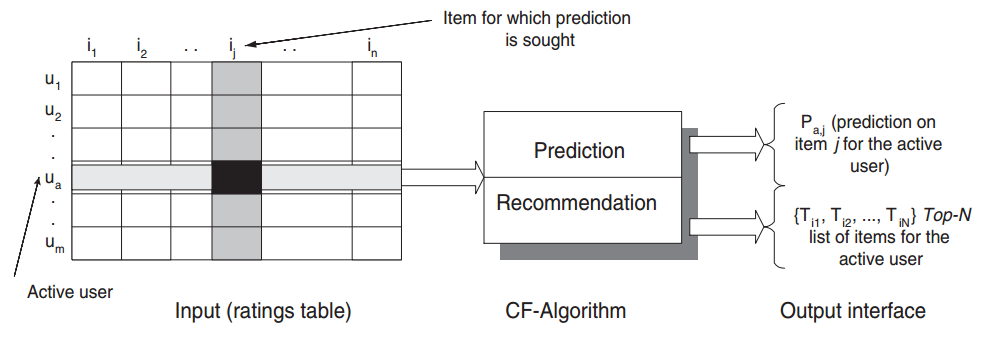
\includegraphics[scale=0.6]{images/collaborative_based.png}
	\end{center}
	\hspace{5.5cm}{Fonte: \citeonline{sarwar2001item}}
\end{figure}

De posse da matriz $n \times m$, o algoritmo \textbf{CF} faz a predição/recomendação ao usuário corrente, demonstrado na figura 2 por $u_{a}$. O usuário $u_{a}$ é visto pelo algoritmo como o alvo atual para o qual serão feitas as predições/recomendações. \citeonline{sarwar2001item} também especificam a predição como um valor numérico que expressa a probabilidade prevista do item ser de interesse do usuário $u_{a}$, sendo este um item ainda não pertencente ao conjunto de $Iu_{a}$. Por outro lado, a recomendação é descrita como uma lista de $\textbf{N}$ itens, cada item $I_{r}$ dentre os itens com a maior probabilidade de utilidade ao usuário ua e ainda não avaliados pelo mesmo. Esta forma de recomendação também é conhecida como recomendação \textbf{Top-N} \cite{adomavicius2005toward}.

Diferentemente do método baseado em conteúdo, a filtragem colaborativa não possui apenas uma abordagem.     Tanto \apudonline{sarwar2001item}{breese1998empirical} quanto \citeonline{adomavicius2005toward} dividem a filtragem colaborativa em duas ramificações:

\begin{itemize}

	\item \textbf{Baseada em memória (\textit{memory-based})}: implica na utilização de toda a matriz $n \times m$ para obter um conjunto de usuários vizinhos (\textit{neighbor-users}), ou seja, usuários que tendem a avaliar diferentes itens similarmente ou itens similares diferentemente ao usuário $u_{a}$. Ao obter o conjunto, os métodos baseados em memória combinam as preferências dos usuários, fornecendo uma recomendação Top-N ao usuário $u_{a}$.

	\item \textbf{Baseada em modelo (\textit{model-based})}: ao invés de utilizar toda a matriz $n \times m$, esta técnica constrói um modelo das avaliações de cada usuário através de diferentes técnicas de \textit{machine learning}, tais como modelos de \textit{cluster} e redes Bayesianas. Devido a complexidade destas técnicas e das mesmas não pertencerem ao escopo da solução apresentada neste trabalho , não abordaremos mais a fundo seu funcionamento.

\end{itemize}

Dessa forma, sistemas de filtragem colaborativa podem ser usados nos casos em que se deseja recomendar itens úteis a um usuário ou fornecer uma previsão ao usuário da probabilidade do mesmo gostar de um item em particular. Além disso, é possível recomendar ao usuário não só itens, mas também usuários ou grupos de usuários que o mesmo possa gostar, o que não é possível nos sistemas baseados em conteúdo \cite{schafer2007collaborative}.

Considerando tais utilidades, tanto \citeonline{schafer2007collaborative} quanto \citeonline{adomavicius2005toward} expõem os sistemas de recomendação baseados em conteúdo e colaborativos como complementares, uma vez que o método baseado em conteúdo prediz a relevância de itens sem avaliações, enquanto o método colaborativo prediz a relevância através de recomendações alheias. A união destas técnicas, em prol de maximizar a eficiência e compensar as limitações (seção 2.2.4), deu origem ao \textbf{método híbrido} que será abordado a seguir.

\subsection{Método Híbrido}

Sistemas de recomendação híbridos seriam quaisquer sistemas que combinam múltiplas técnicas de recomendação para produzir seu resultado \cite{burke2002hybrid, burke2007hybrid}. Como apresentado por \citeonline{adomavicius2005toward}, as técnicas de recomendação possuem limitações de acordo com a abordagem utilizada. Sendo assim, é possível combinar diferentes técnicas para obter o desempenho e precisão desejadas.

\begin{quadro}[h!tp]
	\caption{\label{recommender_systems}Técnicas de recomendação.}

	\begin{center}
		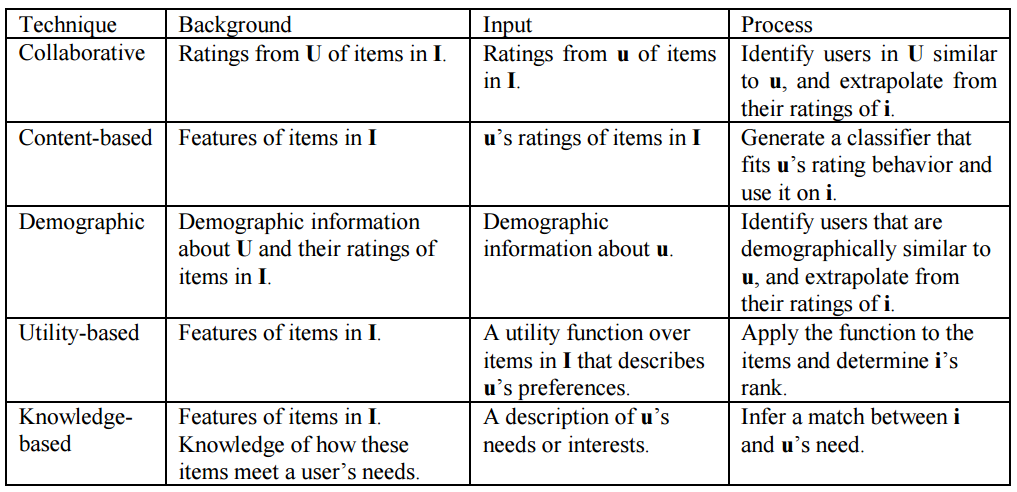
\includegraphics[scale=0.6]{images/recommender_systems.png}
	\end{center}
	\hspace{5.5cm}{Fonte: \citeonline{burke2002hybrid}}
\end{quadro}

Como pode ser visto no quadro 2, \citeonline{burke2002hybrid} apresenta uma série de métodos de recomendação além dos mais comuns abordados neste trabalho. Estes métodos, combinados entre si, podem gerar sistemas híbridos categorizados da seguinte forma:

\begin{itemize}

	\item \textbf{Atribuição de peso (\textit{Weighted}):} Consiste na atribuição de peso para cada um dos métodos empregados no sistema híbrido. Baseado no histórico de acertos entre um método e outro, é possível ajustar o peso de cada um, dando um peso maior ao método atualmente mais eficiente.

	\item \textbf{Escalonamento (\textit{Switching}):} Consiste na utilização de um critério pré-definido para escolher qual método será utilizado no momento. Por exemplo, se o método colaborativo não fornecer uma recomendação com confiança suficiente, o sistema pode trocar para o método baseado em conteúdo.

	\item \textbf{Misto (\textit{Mixed}):} Consiste em usar tanto recomendações de um método quanto de outro, apresentando os resultados de ambos ao usuário.

	\item \textbf{Combinação de características (\textit{Feature Combination}):} Consiste em utilizar a informação colaborativa apenas como características adicionais no conjunto utilizado pelo método baseado em conteúdo.

 	\item \textbf{Cascata (\textit{Cascade}):} Este método em especial consiste em refinamento por estágio, ou seja, o primeiro método é utilizado para gerar um conjunto de recomendações, enquanto o segundo é responsável por refinar o conjunto gerado e assim por diante.

	\item \textbf{Aumento de Recursos (\textit{Feature Augmentation}):} Esta técnica utiliza a recomendação gerada pelo primeiro método como informação para o processamento do segundo método.

	\item \textbf{Meta-nível (\textit{Meta-level}):} Consiste em utilizar o modelo de saída de um método como entrada para o outro. Diferente do aumento de recursos, nesta técnica todo o modelo gerado pelo primeiro método é utilizado.

\end{itemize}

Tendo em vista a taxonomia apresentada por \citeonline{burke2002hybrid}, nota-se que a recomendação híbrida não refere-se ao funcionamento das recomendações, mas sim sobre como os diferentes métodos \textbf{interagem entre si}. Esta interação pode ser insensível à ordem, nos casos de métodos como a atribuição de peso, misto, escalonamento e combinação de características. Já nas outros métodos apresentados, a ordem de execução dos métodos de recomendação alteram o resultado final, uma vez que a saída de um, direta ou indiretamente é a entrada de outro.

Por exemplo, \citeonline{tran2000hybrid} apresentam uma arquitetura híbrida, utilizando os métodos baseado em colaboração (collaborative-based) e baseado em conhecimento (knowledge-based), ambos exemplificados através da arquitetura ilustrada na figura 3.

\begin{figure}[h!tp]

	\caption{\label{hybrid_scheme}Exemplo de arquitetura híbrida.}

	\begin{center}
		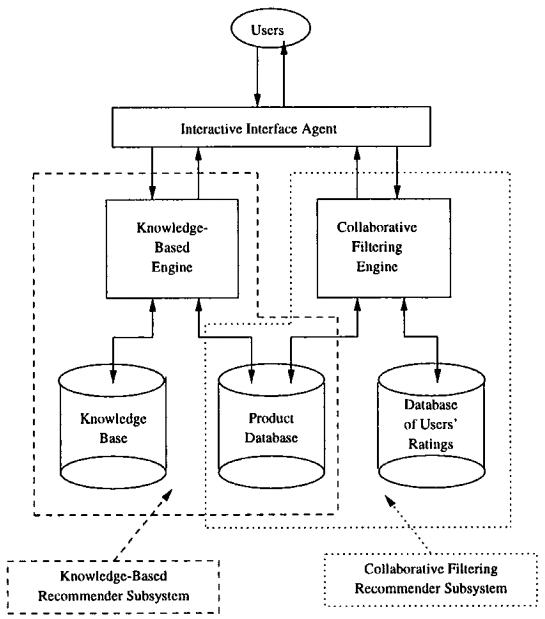
\includegraphics[scale=0.8]{images/hybrid_scheme.png}
	\end{center}

	\hspace{5.5cm}{Fonte: \citeonline{tran2000hybrid}}

\end{figure}

Como ilustrado na figura 3, a arquitetura descrita exemplifica um sistema híbrido de escalonamento (\textit{switching}). Sendo assim, dependendo da situação atual, o sistema pode trocar entre a recomendação colaborativa e a baseada em conhecimento, visando prover melhores recomendações. Considerando que inicialmente a abordagem colaborativa não seria muito eficiente, enquanto a base de dados não possui muitos usuários com modelos conhecidos e não existem itens avaliados o suficiente, \citeonline{tran2000hybrid} optaram por escalonar para o método baseado em conhecimento.

Através dessas limiares, toda vez que o usuário requisita uma recomendação, o agente de interface interativa (\textit{interactive interface agent}) verifica se as mesmas já foram atendidas. Se sim, o agente utiliza a recomendação do método de filtragem colaborativa, se não, o método baseado em conhecimento é utilizado.

Tanto \citeonline{balabanovic1997fab} quanto \citeonline{claypool1999combining} utilizam sistemas híbridos compostos de duas técnicas combinadas: \textbf{baseado em conteúdo} e \textbf{baseado em colaboração}. Dessa forma, é possível utilizar o método colaborativo para gerar o conjunto de $\textbf{N}$ usuários vizinhos (\textit{neighbor-users}) já descrita neste trabalho. A partir do conjunto gerado é aplicado o método baseado no conteúdo destes usuários próximos, aumentando a precisão da recomendação gerada.

Ao invés de se utilizar apenas um método, a utilização de sistemas híbridos pode trazer uma série de benefícios: ao executar recomendações baseadas em conteúdo, o sistema colaborativo pode lidar com novos usuários que ainda não tem seu modelo definido; torna-se possível fazer recomendações precisas a um usuário, mesmo que não existam usuários similares ao mesmo; pode-se recomendar itens não avaliados por nenhum dos usuários, cruzando o modelo dos mesmos com o conteúdo do item \cite{balabanovic1997fab}.

Como forma de verificar a eficácia do método híbrido em relação aos métodos utilizados de forma individual, \citeonline{claypool1999combining} utilizam como métrica a inexatidão, sendo o termo referente a discrepância entre a recomendação obtida e o resultado esperado. A inexatidão dos métodos em relação a seu tempo de utilização pode ser visto através do resultado ilustrado na figura 4.

\begin{figure}[h!tp]
	\caption{\label{innacurace}Inexatidão entre os métodos de recomendação.}
	\begin{center}
		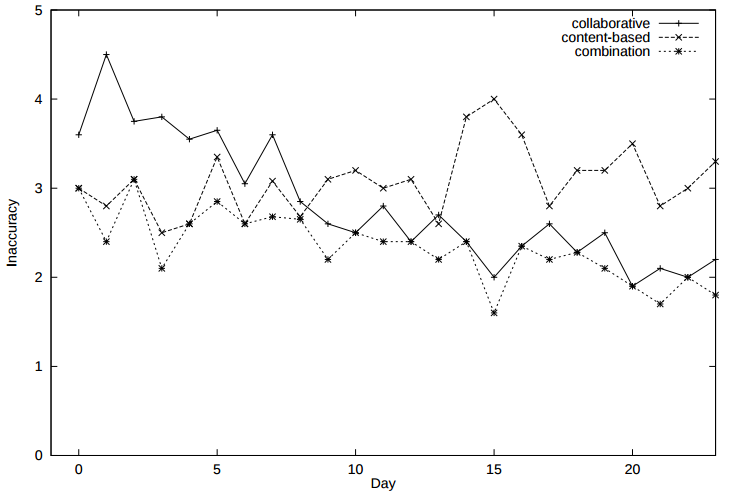
\includegraphics[scale=0.8]{images/innacurace.png}
	\end{center}
	\hspace{5.5cm}{Fonte: \citeonline{claypool1999combining}}
\end{figure}

Analisando a figura 4 pode-se verificar que nos primeiros dias, a inexatidão do método colaborativo era maior devido a falta de completude no modelo dos usuários, construído por meio de usuários que ainda não avaliaram itens, ou de usuários que não se beneficiam da opinião de outros \cite{claypool1999combining}. Conforme o método colaborativo foi estabelecendo relações entre os usuários, este ficou mais preciso e o método baseado em conteúdo começou a ser menos viável. Porém, independente dos picos de inexatidão dos métodos separados mostrados na figura 4, quando combinados (\textbf{recomendação híbrida}), é possível notar uma constância muito maior, possuindo o mais baixo nível de inexatidão em todos os momentos.

Em resumo os sistemas híbridos foram criados para unir técnicas de recomendação com objetivo de \textbf{compensar as limitações} apresentadas pela utilização dessas mesmas técnicas individualmente \cite{balabanovic1997fab}. Tais limitações e seus efeitos no resultado das recomendações serão abordadas na seção a seguir.

\subsection{Limitações}

Conforme apresentado por \citeonline{adomavicius2005toward}, decorrente da utilização das técnicas acima descritas, tanto os sistemas baseados em conteúdo quanto os sistemas colaborativos possuem limitações. Estas limitações, motivo da criação dos sistemas híbridos \cite{balabanovic1997fab}, possuem características claras de acordo com o tipo de recomendação utilizado, sendo divididas da seguinte maneira:

\begin{itemize}

	\item \textbf{Análise de conteúdo limitada (\textit{limited content analysis}):} presente nas técnicas baseadas em conteúdo, devido as mesmas serem limitadas por uma quantidade específica de características relevantes para a recomendação. Além disso, essas características precisam ser extraídas de forma explícita, o que dificulta muito a extração de atributos através de conteúdo como vídeo, imagem, etc.

	\item \textbf{Problema do novo usuario (\textit{new user problem}):} comum nas técnicas que utilizam as preferências do usuário como métrica, consiste no fato de que um usuário precisa ter um número suficiente de avaliações para que o sistema entenda suas preferências e forneça recomendações precisas.

	\item \textbf{Sobre-especialização (\textit{over-specialization}):} comum nas técnicas de recomendação baseada em conteúdo, consiste no fato de que se o sistema apenas recomenda ao usuário itens semelhantes aos que ele já avaliou de forma positiva, o usuário será limitado à apenas recomendações de itens já avaliados, reduzindo cada vez mais a recomendação de novos itens.

	\item \textbf{Problema do novo item (\textit{new item problem}):} sistemas colaborativos baseiam-se apenas nas preferências dos usuários para fazer as recomendações. Sendo assim, novos itens que ainda não foram avaliados por nenhum usuário não serão recomendados.

	\item \textbf{Esparsidade (\textit{Sparsity}):} quando um item é raramente recomendado devido a sua esparsidade no conjunto de usuários e itens, ou seja, um item que é pouco recomendado pelos usuários tende a ser cada vez menos recomendado em sistemas colaborativos, devido ao pouco número de avaliações que o mesmo possui.

\end{itemize}

Sendo assim, grande parte das pesquisas relacionadas a sistemas de recomendação tem como objetivo principal melhorar a precisão das técnicas, reduzindo o impacto das limitações descritas. Porém, como apresentado por \citeonline{mcnee2006being}, nem sempre os itens mais precisos em relação às métricas de cada método são os mais úteis aos usuários.

Considerando que os sistemas de recomendação usualmente abordam apenas algumas, das muitas métricas que definem a utilidade de um item ao usuário, \citeonline{mcnee2006being} ressaltam que cada vez mais a utilização de sistemas de recomendação leva a construção de um conjunto de itens muito similar. Isso ocorre pois quando um usuário avalia um item, as próximas recomendações levarão o mesmo em consideração, recomendando itens cada vez mais parecidos com o item avaliado. Este processo acaba gerando o que \citeonline{mcnee2006being} definem como “\textbf{buraco de similaridade}”, onde o sistema tende a fazer apenas recomendações excepcionalmente similares.

\section{API: \textit{Application Programming Interface}}

Seção sobre API

\subsection{O Padrão RESTful}

Descrever o padrão RESTful

\subsection{Metadados?}

Encaixar os metadados aqui


%
%--------- FIM REFERENCIAL TEORICO------------
%

\chapter{API DE RECOMENDAÇÃO ORIENTADA À METADADOS}

Através dos benefícios da utilização de mais de um método de recomendação em um sistema em forma de serviço, este trabalho propõe o desenvolvimento de uma API Web\footnote{"\textit{Application Programming Interface}" - Conjunto de rotinas e padrões de programação para acesso a um aplicativo de software ou plataforma baseado na Web.} que utiliza metadados\footnote{Dado sobre o dado ou informação sobre a informação.} para fazer a alimentação do conjunto de usuários, itens e avaliações. A combinação destes conjuntos será utilizada para fornecer recomendações às requisições dos clientes.

Partindo da premissa que a API deve atender qualquer modelo de usuário e item, serão fornecidos, em sua inicialização, \textbf{metadados} correspondentes a estrutura de ambos, além da estrutura de avaliação. Assim que os metadados sejam fornecidos à API e os dados sejam fornecidos dentro das estruturas definidas, a requisição de recomendações torna-se simples, uma vez que a API já tem conhecimento do usuário e dos itens avaliados por ele. Este método faz com que o processo de recomendação torne-se \textbf{transparente} ao cliente.

Como forma de recomendação será utilizado o método híbrido, composto dos métodos \textbf{baseado em conteúdo} e \textbf{filtragem colaborativa}, escalonando através do método com melhor precisão momentânea. Dessa forma é possível atender qualquer tipo de metadado, fornecendo recomendações independente do número de usuários, itens e avaliações na base de dados.

De posse das estruturas de metadados fornecidas na inicialização, o cliente poderá alimentar o sistema através das interfaces desenvolvidas na API, constituída pelas funções: \textbf{novos usuários}, \textbf{novos itens} e \textbf{novas avaliações}. Estas três ações de alimentação serão responsáveis por preencher os respectivos conjuntos anteriormente descritos e, a partir deles, construir os modelos de cada usuário para o método colaborativo, bem como a matriz de avaliações para o método baseado em conteúdo. Durante a requisição de uma recomendação, a API definirá o método a ser utilizado e o mesmo fará as recomendações com base nos dados conhecidos, respeitando as propriedades descritas nos metadados.

Em um primeiro momento, a API utilizará o método baseado em conteúdo para fornecer as recomendações e predições, uma vez que poucos itens estarão avaliados e o método colaborativo não terá modelos de usuários suficientes. Assim que as métricas de relações entre usuários e quantidade de modelos processados sejam supridas, a API passará a utilizar o método de filtragem colaborativa, caso este esteja gerando recomendações mais precisas.

Além disso, a API também possuirá a opção do processamento na GPU, agilizando ainda mais o retorno das requisições dos clientes. Este processamento fará uso da tecnologia \textbf{CUDA}, utilizando a GPU nos casos em que seja necessário percorrer a matriz de avaliações, além dos casos de processamento dos modelos de usuários.

\section{Visão Geral}

\section{O Analisador de Dados}

\section{O Motor de Recomendações}

\subsection{Motor de Conteúdo}

\subsection{Motor Colaborativo}

\section{Persistência}

\section{Interface de Usuário}

%
%--------- FIM API------------
%

\chapter{RESULTADOS E DISCUSSÃO}

\chapter{CONSIDERAÇÕES FINAIS}

Devido ao grande número de implementações dos sistemas de recomendação nas mais diversas áreas que aqui foram apresentadas, torna-se notável a vasta gama de aplicações das técnicas e, mais do que isso, a necessidade de um serviço multi-propósito desprendido do uso de linguagens de programação específicas. Sendo assim, ao final do cronograma, espera-se a obtenção de uma API que satisfaça estes requisitos.

Além disso, é importante ressaltar preocupação na construção de uma documentação direta e coesa ao longo de todo o processo, visando uma futura colaboração externa da comunidade, sendo a API de código aberto. Desta forma, o trabalho pode servir não só como uma alternativa \textit{open-source} aos sistemas de recomendação, mas também como uma tecnologia de utilização simples para futuros estudos na área.


\postextual
\bibliography{referencias}
\end{document}








